\section{COMPLEX-Project-1}\label{complex-project-1}

\subsection{\texorpdfstring{\emph{Partie 1 : algorithme approché avec
garantie de
performance}}{Partie 1 : algorithme approché avec garantie de performance}}\label{partie-1-algorithme-approchuxe9-avec-garantie-de-performance}

\paragraph{Question 1}\label{question-1}

Soit \(I\) une instance à notre problème, et \(P\) une permutation
arbitraire des tâches de \(I\), on a :

\[\sum_{i \in I}d_A^i + d_B^i + d_C^i = \sum_{i \in I}d_A^i + \sum_{i \in I}d_B^i + \sum_{i \in I}d_C^i\]

Et la propriété de la somme nous donne :

\[\sum_{i \in I}d_A^i + \sum_{i \in I}d_B^i + \sum_{i \in I}d_C^i \leq 3*max\{\sum_{i \in I}d_A^i, \sum_{i \in I}d_B^i, \sum_{i \in I}d_C^i\} \quad (1)\]

Or nous savons que la durée optimale de notre problème d'ordonnancement
est supérieure ou égale à la somme des durées quelque soit la machine,
soit :
\[max\{\sum_{i \in I}d_A^i, \sum_{i \in I}d_B^i, \sum_{i \in I}d_C^i\} \leq OPT \quad (2)\]

Donc grâce à \((1)\) et \((2)\), nous avons :
\[OPT \geq \frac{\sum_{i \in I}d_A^i + d_B^i + d_C^i}{3}\]

Soit\\\[3 \geq \frac{\sum_{i \in I}d_A^i + d_B^i + d_C^i}{OPT}\]

\(\sum_{i \in I}d_A^i + d_B^i + d_C^i\) est une borne supérieur des
solutions possibles de \(P\). Donc l'ordonnancement associé à P est donc
3-approché.

\paragraph{Question 2 : algorithme de
Johnson}\label{question-2-algorithme-de-johnson}

De même manière que dans la question 1, \(\sum_{i \in I}d_A^i + d_B^i\)
est une borne supérieure aux solutions possibles de la permutation.

On a donc : \[2 \geq \frac{\sum_{i \in I}d_A^i + d_B^i}{OPT}\]

L'ordonnancement obtenu est donc 2-approché.

La complexité de cet algorithme est linéaire, car à chaque itération on
choisit la tâche dont la durée dans la machine A ou dans la machine C
est minimale.

\subsection{\texorpdfstring{\emph{Partie 2 Méthode
exacte}}{Partie 2 Méthode exacte}}\label{partie-2-muxe9thode-exacte}

Conditions Initiales

\begin{itemize}
\itemsep1pt\parskip0pt\parsep0pt
\item
  \(\pi\) = début de la permutation des tâches
\item
  \(t_A^\pi\) = durée pour traiter \(\pi\) tâches sur \(M_A\)
\item
  \(t_B^\pi\) = durée pour traiter \(\pi\) tâches sur \(M_A\) et \(M_B\)
\item
  \(t_C^\pi\) = durée pour traiter \(\pi\) tâches sur \(M_A\) et \(M_B\)
  et \(M_C\)
\end{itemize}

\[ b_A^\pi = t_A^\pi + \sum_{i \in \pi' }d_A^i + min_{i \in \pi'}\{d_B^i + d_C^i\} \]
\(\Rightarrow\) On choisit une tache \(i \in \pi'\) tq \(d_B^i + d_C^i\)
soit min pour " finir rapidement à la fin"

de même manière,

\[b_A^\pi = t_C^\pi + \sum_{ i \in \pi'}d_C^i \]
\[b_B^\pi = t_B^\pi + \sum_{i \in \pi'}d_B^i + min\{d_C^i\}\]

\subsubsection{Question 4}\label{question-4}

soit \(k\) la première tâche de \(\pi'\)

La tache \(k\) ne peut pas commencer dans la machine \(B\) avant sa fin
dans la machine \(A\)

donc

pour \(t_A^\pi + min_{i \in \pi'} \{d_A^i\} > t_B^\pi\)

\[b_B^\pi = t_A^\pi + min_{i \in\pi'} \{d_A^i\}  + \sum_{i \in \pi'}d_B^i + min\{d_C^i\}\]

est toujours une borne inferieure du temps d'execution des tâches.

De même \(t_C^\pi\) est remplacable par
\(max \{t_C^\pi ,t_B^\pi + min_{i \in \pi'}\{d_B^i\}, t_A^\pi +min_{i \in \pi'}\{d_A^i + d_B^i\}\}\)

car la machine C ne peut pas commencer a traiter la tache \(k\) avant
que la fin de son traitement dans la machine B

\subsubsection{Question 5}\label{question-5}

montrez que \(\forall P\) permutation des tâches commençant par \(\pi\)

\(\forall k\in \pi'\)
\[ C_M^P \geq t_A^\pi + (d_A^k+d_B^k+d_C^k) + \sum_{i \in \pi' /k}min\{d_A^i,d_C^i\} \]

\textbf{Réponse}

\begin{itemize}
\item
  \(t_A^\pi\) = durée de la permutation \(\pi\)
\item
  \((d_A^k+d_B^k+d_C^k)\) = durée minimale de la tâche \(k\)
\item
  Il y a 3 cas :
\end{itemize}

\begin{enumerate}
\def\labelenumi{\arabic{enumi}.}
\itemsep1pt\parskip0pt\parsep0pt
\item
  quand k est la première tâche de \(\pi'\)
\item
  quand k est la dernière tâche de \(\pi'\)
\item
  quand k est au milieu
\end{enumerate}

1e cas: on ne compte que \(\{d_C^i\}\) 2e cas : on ne compte que
\(\{d_A^i\}\) 3e cas : on compte \(\{d_A^i\}\) avant la tâche k et
\(\{d_C^i\}\) après la tâche k

\subsubsection{Question 6}\label{question-6}

Avec la Question 5, on a :
\[ b_A' = t_A^\pi + (d_A^k+d_B^k+d_C^k) + \sum_{i \in \pi' /k}min\{d_A^i,d_C^i\} \]
de même manière, on a
\[ b_B' = t_B^\pi + (d_A^k+d_B^k+d_C^k) + \sum_{i \in \pi' /k}min\{d_B^i,d_C^i\} \]

\[ b_C' = t_C^\pi + (d_A^k+d_B^k+d_C^k) + \sum_{i \in \pi' /k } d_C^i \]

\subsubsection{Question 8}\label{question-8}

On peut classer les données en fonction des durées des tâches dans les
machines \(A\), \(B\) et \(C\), ce qui va réduire le temps de recherche
par rapport à une méthode dont l'ordre de recherche des permutations est
aléatoire. Par exemple on peut prioritiser la recherche sur les tâches
dont la durée dans la machine \(A,B\) et \(C\) est la plus petite.

\subsubsection{Question 9}\label{question-9}

Par récurrence on peut trouver tous les minorants \(b_J'\) où J est une
machine quelle conque parmi les \(k\) machines. Donc on peut adapter
cette méthode arborescente à \(k\) machines. Cependant la compléxité
temporelle va augmenter de façon exponentielle (avec chaque machine, le
nombre de noeuds de l'arbre de recherche augemente aussi), donc cette
méthode n'est peut être pas adapté à un nombre \(k\) très grand.

\subsubsection{Question 10}\label{question-10}

Le succès de la méthode dépend essentiellement de la précision de la
fonction d'évaluation. On peut l'accélérer en se contentant d'une
solution approchée avec garantie de qualité. On peut décider d'élaguer
tout nœud dont l'évaluation est inférieure à (1 - \(\alpha\)) fois la
valeur de la meilleure solution courante. Par exemple si \(\alpha\) =
0.05, alors quand on s'arrêtera la valeur de la solution trouvée sera à
moins de 5\% de l'optimum.

\subsection{\texorpdfstring{\emph{Partie 3 : Analyse expérimentale et
étude comparative des différentes
méthodes}}{Partie 3 : Analyse expérimentale et étude comparative des différentes méthodes}}\label{partie-3-analyse-expuxe9rimentale-et-uxe9tude-comparative-des-diffuxe9rentes-muxe9thodes}

\subsubsection{Comparaision entre les deux méthodes
:}\label{comparaision-entre-les-deux-muxe9thodes}

\begin{enumerate}
\def\labelenumi{\arabic{enumi}.}
\itemsep1pt\parskip0pt\parsep0pt
\item
  par rapport au nombre de tâches
\end{enumerate}

\begin{itemize}
\itemsep1pt\parskip0pt\parsep0pt
\item
  La qualité des solutions retournées
\item
  la compléxité temporelle
\end{itemize}

\begin{enumerate}
\def\labelenumi{\arabic{enumi}.}
\setcounter{enumi}{1}
\itemsep1pt\parskip0pt\parsep0pt
\item
  par rapport au nombre de machines
\end{enumerate}

\subsubsection{Test de performance sur les différents types de
tâches}\label{test-de-performance-sur-les-diffuxe9rents-types-de-tuxe2ches}

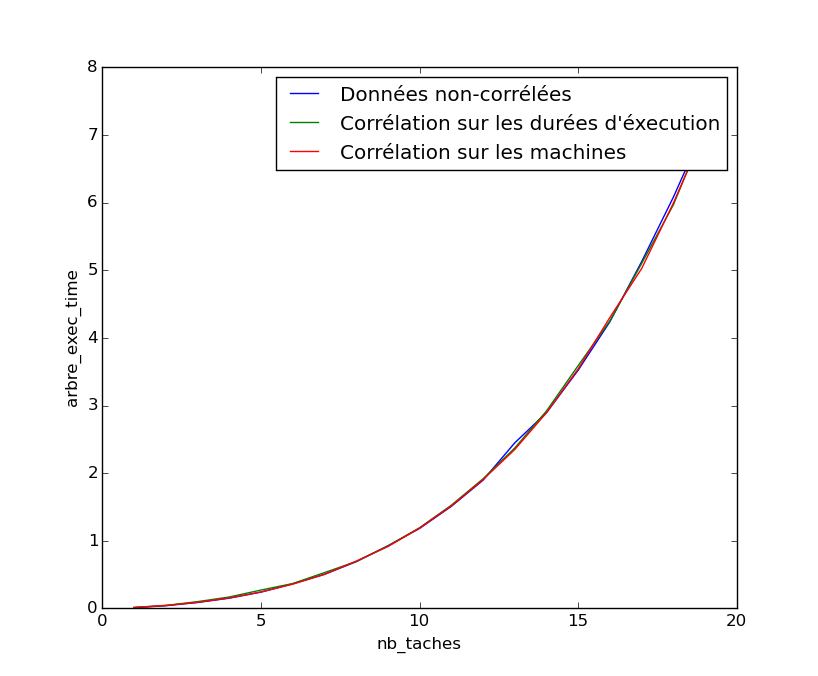
\includegraphics{./arbre_20_3_b1_a4.png}
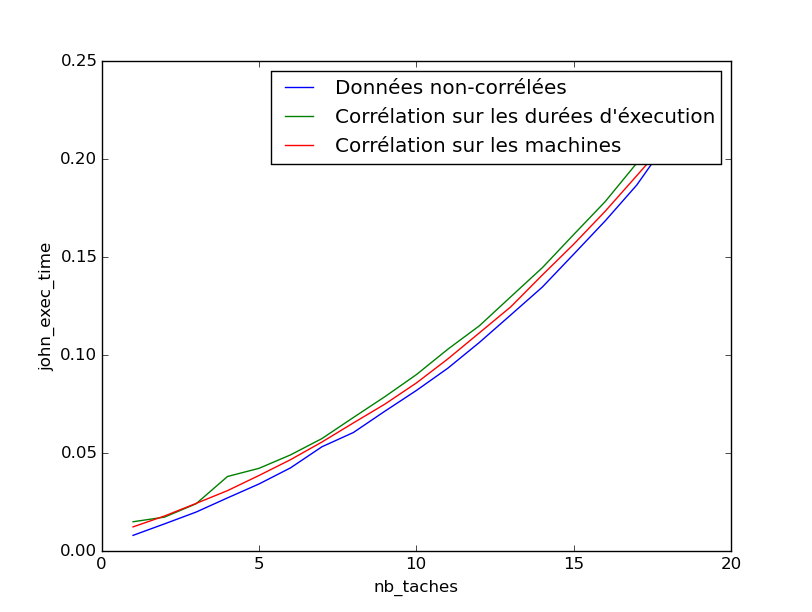
\includegraphics{./john_20_3.png} 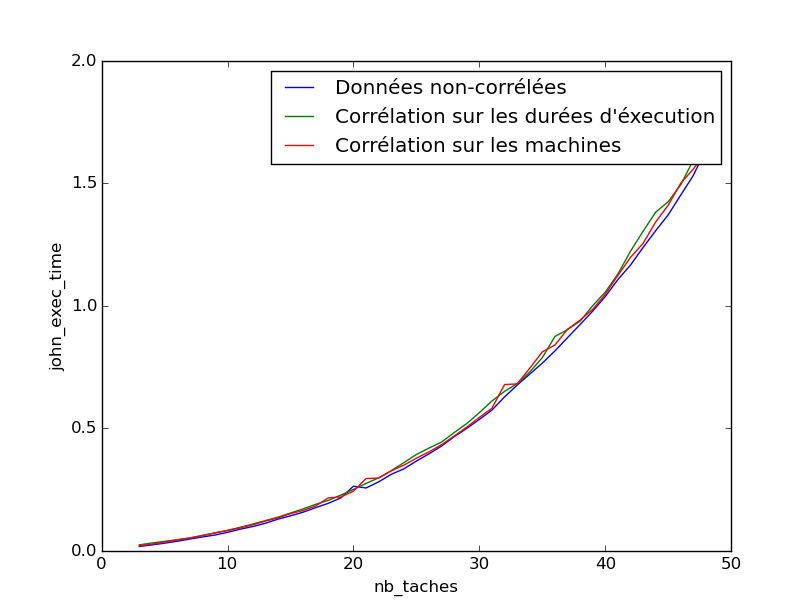
\includegraphics{./john_50_3.png}
